\section{Transport of spinless BECs in speckle potentials}\label{transport}

In Ch.~(\ref{chpt 5}), we study the transport of spinless BECs under speckle potentials. As Fig.~(\ref{fig:single}) shows, a BEC with a chemical potential $\sim 300\ {\rm Hz}$ travels through speckle potentials with average potential depth $\sim 200\ {\rm Hz}$, could be scattered by the speckle potential and decelerate. The deceleration of a BEC depends on its initial velocity, the speckle potential depth, and the cutoff $k_c$ in the speckle potential PSD. As Fig.~\ref{fig:single}(d) shows, after evolving under the speckle potentials for $16\ {\rm mm}$, the BECs with small initial velocity has more significant deceleration. For BECs with large initial velocity, $k_0>k_c/2$, the deceleration is minimal during the $16\ {\rm mm}$.

In the experiments, we study how BECs with different velocities decelerate. As discussed in Ch.~(\ref{speckle_chapter}), we can make speckle potentials that have the same PSD as the ones we use in our numerical simulations. And as discussed in Sec.~(\ref{speckle_pulsing}), the average speckle potential depth can be inferred from a PD reading. So an ideal experimental sequence is to have the BEC travel with constant velocity under well-calibrated speckle potential, and the final velocity would be measured by using $insitu$ or TOF absorption images. To that end, the first challenge we are faced with is that how to make a BEC travel with a constant velocity for an extensive amount of time ($16\ {\rm mm}$ in the simulation). We make BECs by doing evaporative cooling in a cross dipole trap as discussed in Sec.~(\ref{dipole trap}), so our first choice is to make BECs travel in the cross dipole trap. As Eq.~(\ref{dipole_poten}) suggests, dipole potential is proportional to the intensity of the dipole beam. 

In our case, as discussed in \ref{speckle_design}, we image atoms in $z$ direction and measure the motion of atoms in $x$ direction. The dipole potential in $x$ direction is a combination of the dipole potential from $z$ dipole beam and $x$ dipole beam. The width of the dipole potential from $x$ dipole beam is the Rayleigh range, which in our case is $\sim 1.3\ {\rm mm}$. Based on our design, the velocity of atoms corresponds to the recoil $k$ vector $k_r$ is $3.3\ {\rm \mu m/ms}$. We expect the atoms to move less than $50\ {\rm \mu m}$ during the experiment, so the dipole potential from x dipole beam can be ignored.

In $x$ direction, the dipole potential from the $z$ dipole beam is
\begin{equation}
    V_{dip}(x) = -V_0\exp{-\frac{2x^2}{w^2}}.
\end{equation}
where $w$ is the width of the beam at the atoms. Expand the potential at $x=0$ to second order,
\begin{equation}
    V_{dip}(x) \approx -V_0 + \frac{2V_0}{w^2}x^2,
\end{equation}
has a quadratic form. Around the center of the trap, the dipole potential can be approximated by a harmonic potential with frequency $\sqrt{\frac{4V_0}{w^2}}$.

In the ideal case, the atoms would move at a constant velocity in the dipole trap, meaning the frequency $\sqrt{\frac{4V_0}{w^2}}$ is zero and the $z$ dipole beam is completely turned off. More realistically, if the velocity of the atoms change by less than 5\% at the center of the trap in $15\ {\rm ms}$, the period of the harmonic oscillation needs to be more than $300\ {\rm ms}$. So the trapping frequency is around $3\ {\rm Hz}$. 

The $x$ dipole beam and the $z$ dipole beam in our experiments are the first order and zeroth-order beams from an AOM, the total power of the two beams are conserved. We optimized the ratio of the power of the two beams to maximize the phase space density of the BECs after the dipole evaporation stage. In the optimized case, the measured trapping frequency in $x$ direction is $21\ {\rm Hz}$. In order to decrease the $x$ trapping frequency, we need to allocate more power in the $x$ dipole beam and less in the $z$ dipole beam. But in the process of decreasing the $x$ trapping frequency, a few problems occurred. 

Fig.~\ref{fig:lower trapping freq} shows the BEC with $x$ trapping frequency of $21\ {\rm Hz}$ compared with the BEC with $x$ trapping frequency of $5.8\ {\rm Hz}$. Compared with the BEC in Fig.~\ref{fig:lower trapping freq}(a), the BEC in Fig.~\ref{fig:lower trapping freq}(b) is stretched in the $x$ direction due to small trapping frequency. The signal is much weaker and the large length in $x$ direction makes it hard to accurately detect the center of the atoms and the center-of-mass motion.

\begin{figure*}
    \centering
    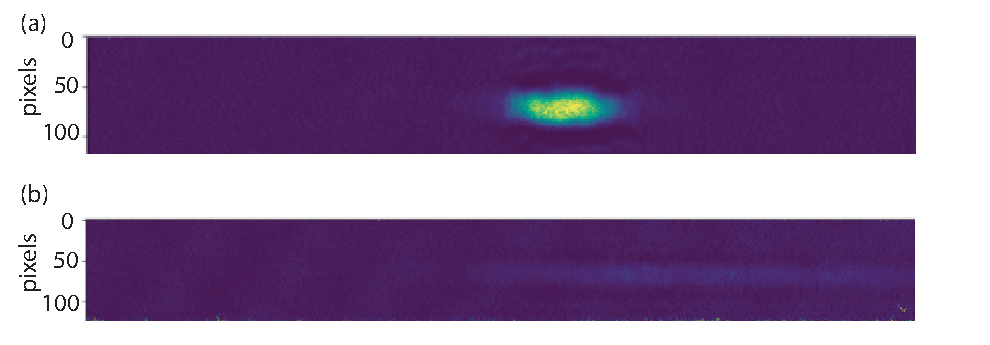
\includegraphics{Chapter6_secs/decrease_trap_freq.pdf}
    \caption{$insitu$ absorption images of BECs with different dipole parameters. (a) A BEC with $x$ trapping frequency of $21\ {\rm Hz}$. (b) A BEC with $x$ trapping frequency of $5.8\ {\rm Hz}$}
    \label{fig:lower trapping freq}
\end{figure*}

Alternatively, we can keep the current dipole trap configuration and decrease the time that BECs travel under speckle potentials. We hope to find the duration of the speckle potential pulses that is as short as possible, but its deceleration effect on the BECs is still significant for speckle potential weak enough not to cause trapping effect. 

In Fig.~\ref{fig:deceleration_in_dip_osc}, the blue dots show the oscillation of a BEC in $x$ direction in a dipole trap with $x$ trapping frequency $21\ {\rm Hz}$. The center of the atoms is measured from $insitu$ images of atoms. At the center of the dipole trap, the atoms are at the maximum velocity $v_0$, $mv_0/\hbar = 1.8k_r$. The first time the atoms reach maximum velocity is at $21\ {\rm ms}$. We make the atoms do the same dipole oscillation as the blue dots show, at $21\ {\rm ms}$, we turn on the speckle potential and hold for $1\ {\rm ms}$. After $1\ {\rm ms}$, the speckle potential is turned off and we track the center-of-mass motion of the atoms in $x$ direction in the dipole trap. The center-of-mass motion of atoms after the speckle pulse is shown as the orange dots in Fig.~\ref{fig:deceleration_in_dip_osc}. 

\begin{figure*}
    \centering
    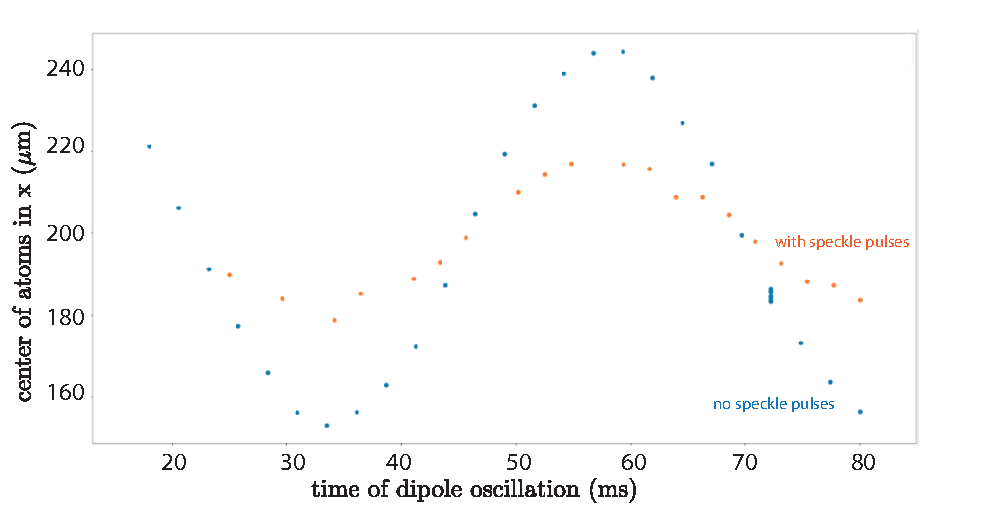
\includegraphics{Chapter6_secs/deceleration_in_dip_osc.pdf}
    \caption{Center-of-mass motion in $x$ direction of atoms during dipole oscillation. The blue dots show a full cycle of dipole oscillation without pulses of the speckle potentials. The orange dots show the dipole oscillation of atoms with the same initial velocity as the blue dots show, but with a $1\ {\rm ms}$ speckle pulse at $21\ {\rm ms}$. The average speckle potential depth is $\approx 640\ {\rm Hz}$.}
    \label{fig:deceleration_in_dip_osc}
\end{figure*}

The amplitude of the oscillation shown by the orange dots is smaller than the amplitude shown by the blue dots. We fit a sinusoidal function to both and infer the velocities of the atoms at $t=21\ {\rm ms}$. Without the pulse of speckle potential at $t=21\ {\rm ms}$, the velocity of the atoms is $v_0$, $mv_0/\hbar = 1.8k_r$. With the pulse, the velocity of the atoms is $v_f$, $mv_f/\hbar = 0.7k_r$. This measurement demonstrated that a speckle potential pulse with an average potential depth of $\approx 640\ {\rm Hz}$, can have a significant deceleration effect on atoms within $1\ {\rm ms}$. This allows us to measure the deceleration of atoms evolving in speckle potentials in our optimized dipole trap, without having to reduce the $x$ trapping frequency.

Using this method, we measured the deceleration of atoms at different velocities $v_0$ after pulses of speckle potential for $1\ {\rm ms}$ with an average potential depth of $\approx 500\ {\rm Hz}$. Fig.~\ref{fig:spinless transport} shows the experimental measurements compared with the numerical simulation results. The red circles in Fig.~\ref{fig:spinless transport} show the experimental results. In the numerical simulations, we make atoms with different initial velocities evolve under speckle potentials with different potential depth for $1\ {\rm ms}$ and measure the final velocities. The initial velocities range from $0.2\frac{\hbar k_r}{m}$ to $2.2\frac{\hbar k_r}{m}$. The blue curve and the yellow curve in Fig.~\ref{fig:spinless transport} correspond to speckle potential depth of $500\ {\rm Hz}$ and $800\ {\rm Hz}$, respectively. In the experiments, the average speckle potential depth is inferred from Fig.~\ref{fig:avg_speckle_poten}. As discussed in Sec.~\ref{long_pulse}, we use the stationary width of the momentum distribution after long-term speckle pulses to measure the average speckle potential. Here the deceleration measurement is done with a PD reading of $1.0\ {\rm V}$, which corresponds to an average speckle potential of $\approx 500\ {\rm Hz}$. For initial velocities $v_0$, the measured final velocities $v_f = \frac{\hbar k_r}{m}$ are lower than the final velocities in the simulation with average speckle potential of $500\ {\rm Hz}$, and are close to those in the simulation with average speckle potential of $800\ {\rm Hz}$. There are a few potential causes that can lead to the gap. First, in the measurements of the stationary width of momentum distribution after long-term pulses of speckle potential shown in Fig.~\ref{fig:avg_speckle_poten}, the stationary width is noisy which leads to uncertainty in the calculation of average speckle potential depth. Second, as discussed in Sec.~\ref{short_pulse_sec}, it is hard to measure the $k_c$ of the optical speckle potentials used in the experiments accurately. The difference in $k_c$ of speckle potentials used in the simulations and the experiments can also lead to this gap.

%we fit a Gaussian function to the spatial distribution of atoms to extract the center-of-mass positions, as the dots in Fig.~\ref{fig:deceleration_in_dip_osc} show. Then we fit a sinusoidal function to the center-of-mass positions of atoms when they oscillate in a dipole trap, and infer the velocity at $t=21~{\rm ms}$. The Gaussian fits and the inference of velocities from the sinusoidal fits also introduce uncertainties.

\begin{figure*}
    \centering
    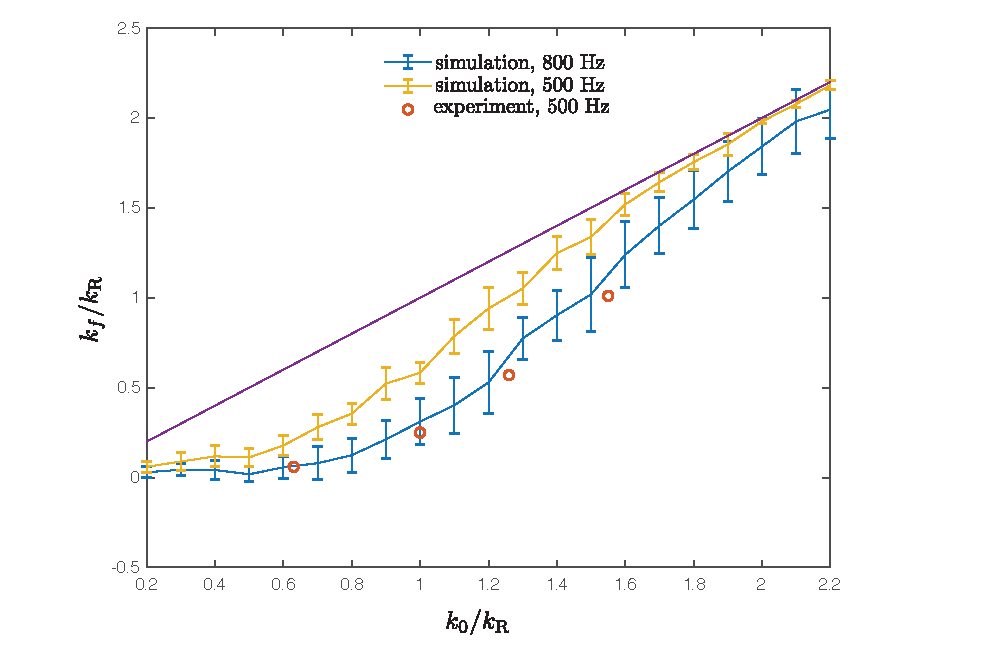
\includegraphics{Chapter6_secs/spinless_transport.pdf}
    \caption{Deceleration of atoms after a $1\ {\rm ms}$ pulse of the speckle potentials. The red circles are the results of measurements in the experiments. The average speckle potential depth inferred from the photo diode reading is $\approx 500\ {\rm Hz}$. The blue curve and the yellow curve are the results of numerical simulations. The blue curve is the final velocities vs the initial velocities after evolving under speckle potentials with average potential depth of $800\ {\rm Hz}$, and the yellow curve is for speckle potential with average potential depth of $500\ {\rm Hz}$. Both the blue curve and the yellow curve are averaged over 20 speckle realizations and the error bars show the standard deviations. The purple line is diagonal. }
    \label{fig:spinless transport}
\end{figure*}